\documentclass[12pt]{article}
\usepackage{indentfirst}
\usepackage{siunitx}
\usepackage{graphicx}
\usepackage{subfigure}
\usepackage{float}

\setlength{\parindent}{20pt}
\setlength{\oddsidemargin}{0.5cm}
\setlength{\evensidemargin}{0.5cm}
\setlength{\marginparsep}{0.75cm}
\setlength{\marginparwidth}{2.5cm}
\setlength{\marginparpush}{1.0cm}
\setlength{\textwidth}{150mm}
\setlength{\parindent}{1cm}

\begin{document}
	\begin{titlepage}
		\vspace*{\stretch{1.0}}
		\begin{center}
			\Large\textbf{Conservation of Momentum}\\
			\Large\textmd{WU, Chenhao}\\
			\Large\textmd{Student ID: 117010285}\\
			\Large\textmd{October 19th, 2018}
		\end{center}
		\vspace*{\stretch{2.0}}
	\end{titlepage}

	\section{Objective}
	In this experiment, we tried to verify the conservation of momentum using two dynamics carts of different masses. We performed both elastic collisions and inelastic collisions, and we tried to show that in both cases, momentum is conserved.\par
	Cart velocities are recorded using two Rotary Motion Sensors connected to the carts by string wrapped around pulleys. This measurement method adds very little friction to the experiment and, since the velocities are continuously monitored, any deceleration due to friction can be measured. The total kinetic energy before and after the collision is also studied.
	
	\section{Theory}
	The momentum of a cart depends on its mass and velocity.
	\begin{equation}
		Momentum = p = mv
	\end{equation}\par
	The direction of the momentum is the same as the direction of the velocity. During a collision, the total momentum of the system of both carts is conserved because the net force on the two-cart system is zero. This means that the total momentum just before the collision is equal to the total momentum just after the collision. If the momentum of one cart decreases, the momentum of the other cart increses by the same amount. This is true regardless of the type of collision, and even in cases where kinetic energy is not conserved. The law of conservation of momentum is stated as
	\begin{equation}
		p_{TotalBeforeCollision} = p_{TotalAfterCollision}
	\end{equation}\par
	The kinetic energy of a cart also depends on its mass and speed but kinetic energy is a scalar.
	\begin{equation}
		K_E = \frac{1}{2}mv^{2}
	\end{equation}\par
	The total kinetic energy of the system of two carts is found by adding the kinetic energies of the individual carts.
	
	\section{Experiment Procedures}
	\subsection{Setup}
		Before the experiment, we need to guarantee the track has levelled horizontally. We levelled the track using the leveling screws on the track feet til after placing a car at rest on the track, the car won't gain any acceleration in either direction while being given a little push. \par
		After then we measured the mass of each cart including the string bracket on each cart. \par
		Since we need to use Rotation Motion Sensors to measure the velocity of carts, we attached a line of thread to each cart using the string bracket. The thread was run over the largest pulley on the Rotary Motion Sensor and then over the small pulley on the end of the track, then return to the string bracket on the cart. \par 
		In the end, we plugged the Rotary Motion Sensor attached to the red cart into Channels P1 on the 550 interface and plug the Rotary Motion Sensor attached to the blue cart into Channels P2 on the interface, and then we configured the Capstone software til the Capstone can catch the return from sensors and display the data we want. \par 
	\subsection{Experiment 1. Explosions}
		\subsubsection{Explosion between Equal Mass Carts}
		1. Depress the plunger on one cart to position 2. Place the two carts in contact with each other in the center of the track. \par
		2. Start recording and tap the trigger release to launch the carts. Hitting the trigger with a mass bar works well. \par
		3. Stop recording before either cart reaches the end of the track. \par 
		4. Record the velocities of two carts just after explosion. \par 
		\subsubsection{Explosion between Unequal Mass Carts}
		1. Measure the mass of two mass bars and then place them both in one cart that won't be depressed the plunger. \par 
		2. Depress the plunger on one cart to position 2. Place the two carts in contact with each other in the center of the track. \par 
		3. Start recording and tap the trigger release to launch the carts. Hitting the trigger with a mass bar works well. \par 
		4. Stop recording before either cart reaches the end of the track. \par 
		5. Record the velocities of two carts just after explosion. \par 
	\subsection{Experiment 2. Completely Inelastic Collisions}
		\subsubsection{Completely Inelastic Collision between Equal Mass Carts}
		1. Place two carts at rest on the track with some distance with each other. Direct the bumpers facing each other. \par
		2. Start recording and give one cart a push toward the other cart. In inelastic collision, two carts will stick to each other and move together after the collision. \par 
		3. Stop recording before either cart reaches the end of the track. \par 
		4. Record the velocities of two carts before and just after explosion. \par 
		\subsubsection{Completely Inelastic Collision between Unequal Mass Carts}
		1. Measure the mass of two mass bars and then place them both in one cart that won't be initially pushed. \par 
		2. Place two carts at rest on the track with some distance with each other. Direct the bumpers facing each other. \par
		3. Start recording and give one cart a push toward the other cart. In inelastic collision, two carts will stick to each other and move together after the collision.\par 
		4. Stop recording before either cart reaches the end of the track. \par 
		5. Record the velocities of two carts before and just after explosion. \par 
	\subsection{Experiment 3. Elastic Collisions}
		\subsubsection{Elastic Collision between Equal Mass Carts}
		1. Place two carts at rest on the track with some distance between each other, and then direct the magnetic bumpers facing each other. \par 
		2. Start recording and give one cart a push toward the other cart. \par 
		3. Stop recording before either cart reaches the end of the track. \par 
		4. Record the velocities of both two carts just after the collision, and record the velocity of the cart had been pushed before the collision. \par 
	    \subsubsection{Elastic Collision between Unequal Mass Carts}
	    1. Measure the mass of two mass bars and then place them both in one cart that won't be initially pushed. \par 
	    2. Place two carts at rest on the track with some distance between each other, and then direct the magnetic bumpers facing each other. \par 
	    3. Start recording and give one cart a push toward the other cart. \par 
	    4. Stop recording before either cart reaches the end of the track. \par 
	    5. Record the velocities of both two carts just after the collision, and record the velocity of the cart had been pushed before the collision. \par 
	 
	\section{Experimental Data}
	\subsection{Error Estimation}
	The data we obtained include: velocity of carts by Rotary Motion Sensors, mass of all objects.
		\begin{itemize}
			\item Velocity: the error is mainly due to the instrument error. According to the manual of Rotary Motion Sensors (PS-2120A), the resolution of the equipment is $0.09^\circ$(angular) at 4,000 points per revolution. Therefore, the error we estimated is about $\SI{\pm0.00157}{{\radian}/{\second}}$.
			\item Mass: the scale has as resolution of $\SI{0.01}{\gram}$, so the estimated error is $\SI{\pm0.01}{\gram}$ 
		\end{itemize}
	\subsection{The Raw Data}
		\subsubsection{Raw Data of Experiment 1}
		\begin{figure}[H]
			\centering
			\subfigure{}{
			\label{Fig. Experimental Data of Ex.1}
			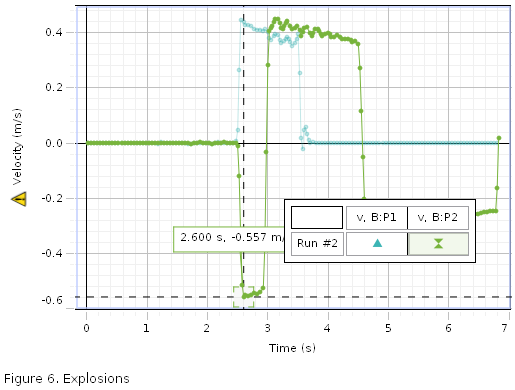
\includegraphics[width=0.4\textwidth, height=0.3\linewidth]{/home/vitowu/Documents/e3/Journal8.png}
			\includegraphics[width=0.4\textwidth, height=0.3\linewidth]{/home/vitowu/Documents/e3/Journal5.png}
			\includegraphics[width=0.8\textwidth, height=0.2\linewidth]{/home/vitowu/Documents/e3/Journal2.png}}
		\end{figure}
		\subsubsection{Raw Data of Experiment 2}
		\begin{figure}[H]
			\centering
			\subfigure{}{
				\label{Fig. Experimental Data of Ex.2}
				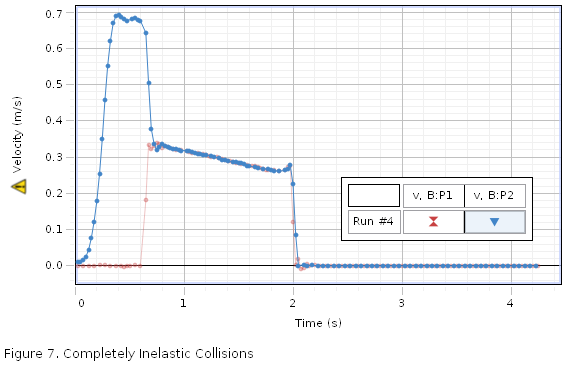
\includegraphics[width=0.4\textwidth, height=0.3\linewidth]{/home/vitowu/Documents/e3/Journal9.png}
				\includegraphics[width=0.4\textwidth, height=0.3\linewidth]{/home/vitowu/Documents/e3/Journal6.png}
				\includegraphics[width=0.8\textwidth, height=0.2\linewidth]{/home/vitowu/Documents/e3/Journal3.png}}
		\end{figure}
		\subsubsection{Raw Data of Experiment 3}
		\begin{figure}[H]
			\centering
			\subfigure{}{
				\label{Fig. Experimental Data of Ex.3}
				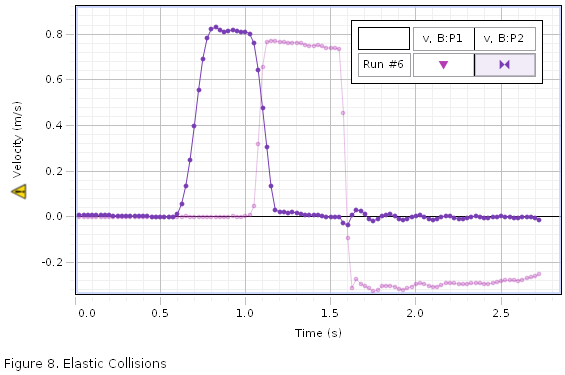
\includegraphics[width=0.4\textwidth, height=0.3\linewidth]{/home/vitowu/Documents/e3/Journal10.png}
				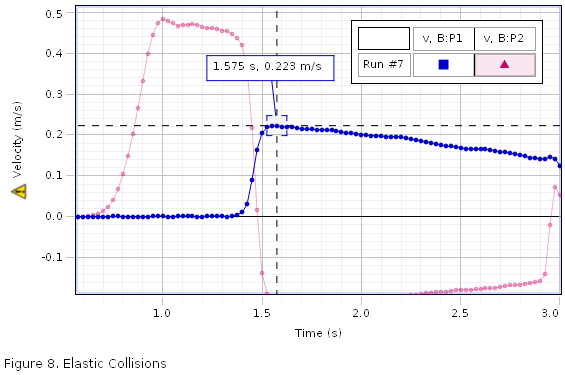
\includegraphics[width=0.4\textwidth, height=0.3\linewidth]{/home/vitowu/Documents/e3/Journal7.png}
				\includegraphics[width=0.8\textwidth, height=0.2\linewidth]{/home/vitowu/Documents/e3/Journal4.png}}
		\end{figure}
	
	\section{Data and Error Analysis}
	\subsection{Data Calculation}
		\subsubsection{Momemtum}
		According to equation(1), we can use mass and velocity of an object to calculate its momentum. Therefore, the error of the calculated momentum is that,
		\begin{equation}
			\delta p = \sqrt{(\frac{\partial p}{\partial m})^2(\delta m)^2 + (\frac{\partial p}{\partial v})^2(\delta v)^2}
		\end{equation} \par 
		Then we can calculate all the momentums we want,
		\begin{table}[H]
			\centering
			\makebox[\linewidth]{
			\begin{tabular}{|c|c|c|c|c|c|c|}
				\hline
				\hline
				Collision Type & $p_{RedInit}$  & $p_{BlueInit}$ & $\sum p_{Init}$ & $p_{RedFinal}$ & $p_{BlueFinal}$ & $\sum p_{Final}$ \\
				\hline
				Equal Mass Explosion & 0$\pm0.0042$ & 0$\pm0.0042$ & 0$\pm0.0084$ & 147.37$\pm0.15$ & -117.32$\pm0.13$ & 30.05$\pm0.28$ \\
				\hline
				Unequal Mass Explosion & 0$\pm0.0042$ & 0$\pm0.012$ & 0$\pm0.0162$ & 97.10$\pm0.097$ & -135.49$\pm0.012$ & -38.39$\pm0.109$ \\
				\hline
				Equal Mass Inelastic & 182.02$\pm0.042$ & 0$\pm0.0042$ & 182.02$\pm0.0462$ & 87.04$\pm0.042$ & 86.54$\pm0.041$ & 173.58$\pm0.083$ \\
				\hline
				Unequal Mass Inelastic & 164.03$\pm0.042$ & 0$\pm0.0042$ & 164.03$\pm0.0462$ & 40.74$\pm0.42$ & 118.55$\pm0.53$ & 159.29$\pm0.95$ \\
				\hline
				Equal Mass Elastic & 214.04$\pm0.042$ & 0$\pm0.0042$ & 214.04$\pm0.0462$ & 4.76$\pm0.042$ & 202.80$\pm0.41$ & 205.56$\pm0.452$ \\ 
				\hline
				Unequal Mass Elastic & 119.85$\pm0.42$ & 0$\pm0.0042$ & 119.85$\pm0.4242$ & -56.09$\pm0.42$ & 171.67$\pm1.21$ & 115.58$\pm1.63$ \\
				\hline
			\end{tabular}
		}
			\bigskip
			All variables calculated above have Units $\SI{}{\kilogram*\meter/\second}$
		\end{table}
		Further more, we can continue to calculate the difference between the momentum before collision and after collision, and we obtain a table as following,
		\begin{table}[H]
			\centering
			\makebox[\linewidth]{
			\begin{tabular}{|c|c|}
				\hline
				\hline
				Collision Type & $\frac{p_{before}-p_{after}}{p_{before}}\times100\%$ \\
				\hline
				Equal Mass Inelastic & 4.64\% \\
				\hline
				Unequal Mass Inelastic & 2.89\% \\
				\hline
				Equal Mass Elastic & 3.96\% \\
				\hline
				Unequal Mass Elastic & 3.56\% \\
				\hline
			\end{tabular}
			}
		\end{table}
		
		\subsubsection{Kinetic Energy}
		According to Equation(3), we can use mass and velocity of an object to calculate its kinetic energy. Therefore the error of the calculated momentum is that,
		\begin{equation}
		\delta KE = \sqrt{(\frac{\partial KE}{\partial m})^2(\delta m)^2 + (\frac{\partial KE}{\partial v})^2(\delta v)^2}
		\end{equation} \par
		
		\begin{table}[H]
			\centering
			\makebox[\linewidth]{
				\begin{tabular}{|c|c|c|c|c|c|c|}
					\hline
					\hline
					Collision Type & $KE_{RedInit}$  & $KE_{BlueInit}$ & $\sum KE_{Init}$ & $KE_{RedFinal}$ & $KE_{BlueFinal}$ & $\sum KE_{Final}$ \\
					\hline
					Equal Mass Explosion & 0 & 0 & 0 & 41.04$\pm0.23$ & 26.16$\pm0.18$ & 67.2$\pm0.41$ \\
					\hline
					Unequal Mass Explosion & 0 & 0 & 0 & 17.82$\pm0.153$ & 4.07$\pm0.073$ & 21.89$\pm0.226$ \\
					\hline
					Equal Mass Inelastic & 62.62$\pm0.29$ & 0 & 62.62$\pm0.29$ & 14.32$\pm0.14$ & 14.24$\pm0.14$ & 28.56$\pm0.28$ \\
					\hline
					Unequal Mass Inelastic & 50.85$\pm0.26$ & 0 & 50.85$\pm0.26$ & 3.14$\pm0.064$ & 9.13$\pm0.19$ & 12.27$\pm0.254$ \\
					\hline
					Equal Mass Elastic & 86.58$\pm0.34$ & 0 & 86.58$\pm0.34$ & 0.043$\pm0.0075$ & 78.18$\pm0.32$ & 78.223$\pm0.3275$ \\ 
					\hline
					Unequal Mass Elastic & 27.15$\pm0.19$ & 0 & 27.15$\pm0.19$ & 5.95$\pm0.088$ & 19.14$\pm0.27$ & 25.09$\pm0.358$ \\
					\hline
				\end{tabular}
			}
			\bigskip
			All variables calculated above have Units $\SI{}{\J}$
		\end{table}
		As what we did before, we can continue to calculate the difference between the kinetic energy before and after collision, and we obtain a table as following,
		\begin{table}[H]
			\centering
			\makebox[\linewidth]{
				\begin{tabular}{|c|c|}
					\hline
					\hline
					Collision Type & $\frac{KE_{before}-KE_{after}}{KE_{before}}\times100\%$ \\
					\hline
					Equal Mass Inelastic & 54.39\% \\
					\hline
					Unequal Mass Inelastic & 75.87\% \\
					\hline
					Equal Mass Elastic & 2.93\% \\
					\hline
					Unequal Mass Elastic & 7.59\% \\
					\hline
				\end{tabular}
			}
		\end{table}
	\subsection{Plot}
	After all the experimental data have been collected, we'd like to plot the experimental data in order to present the relationship between variables more intuitively.
	\subsubsection{Experiment 1. Explosion}
	\begin{figure}[H]
		\centering
		\subfigure{}{
			\label{Fig. Experimental Plot of Ex.1}
			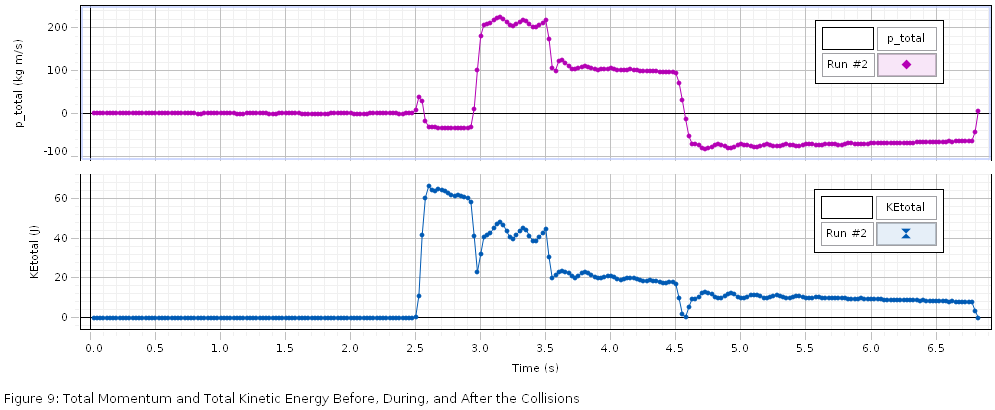
\includegraphics[width=0.4\textwidth]{/home/vitowu/Documents/e3/an/Journal1.png}
			\includegraphics[width=0.4\textwidth]{/home/vitowu/Documents/e3/an/Journal4.png}
		}
	\end{figure}
	We can observe from the plot that both the momentum and the kinetic energy of the 2-carts system reduced after explosion.
	\subsubsection{Experiment 2. Inelastic Collision}
	\begin{figure}[H]
		\centering
		\subfigure{}{
			\label{Fig. Experimental Plot of Ex.2}
			\includegraphics[width=0.4\textwidth]{/home/vitowu/Documents/e3/an/Journal2.png}
			\includegraphics[width=0.4\textwidth]{/home/vitowu/Documents/e3/an/Journal5.png}
		}
	\end{figure}
	We can observe from the plot that the momentum kept conservation after collision, while the kinetic energy reduced after inelastic collision.
	\subsubsection{Experiment 3. Elastic Collision}
	\begin{figure}[H]
		\centering
		\subfigure{}{
			\label{Fig. Experimental Plot of Ex.3}
			\includegraphics[width=0.4\textwidth]{/home/vitowu/Documents/e3/an/Journal3.png}
			\includegraphics[width=0.4\textwidth]{/home/vitowu/Documents/e3/an/Journal6.png}
		}
	\end{figure}
	We can observe from the plot that both the momentum and the kinetic energy kept conservation after elastic collision.
	
	\section{Conclusion}
	During the experiment, we tried to verify the conservation of momentum in different type of collisions. The friction on track and the force while releasing the plunger may slightly cause the bias and random error of collected data. Yet, the operations and procedures can be more accurate. From the data collected so far, however, the result matches the theory and our expectation, which means that we've verified following thesis:
	\begin{itemize}
		\item For Inelastic Collision: the momentum holds conservation while kinetic energy does not.
		\item For Elastic Collision: both the momentum and the kinetic energy hold conservation after collision. 
		\item Addition: Two carts swap their velocities after elastic collision with equal mass.
	\end{itemize}
	
\end{document}